
% !TeX program = xelatex
\documentclass[a4paper]{scrarticle}

\usepackage{../paper/style}
\usepackage{pdfpages}

\geometry{left=2.25cm, right=2.25cm, top=4.0cm, bottom=4.00cm}

\ihead{Evaluationsblatt Modelvalidierung \textbf{Algo}rithmische Ski\textbf{tour}enplanung Algotour~---~algotour.app}
\ifoot{\\Jesse Born, 2024}

\begin{document}
\subsection*{Persönliche Angaben Evaluationsperson}
\smallskip
\smallskip
\begin{center}
  
  \begin{tabular}{ l l }
    Name: \line(1,0){150}  & Vorname: \line(1,0){150} \\[15pt]
    Adresse: \line(1,0){150}  & Email: \line(1,0){150} \\[15pt]
    Ausbildung: & \\[5pt]
    $\square$ Bergführer & $\square$ Bergführeraspirant \\[5pt]
    $\square$ SAC-Tourenleiter & $\square$ Freizeittourengänger \\[5pt]
    $\square$ Skilehrer mit Modul Varianten+Touren & $\square$ Sonstige (J+S Skitouren, Skilehrer S+R etc.) \\[5pt]
  \end{tabular}
\end{center}

\hrule
\subsection*{Anleitung}

\begin{itemize}
  \item Orientiere dich auf dem Kartenabschnitt
  \item Folge der Route, vermerke alpintechnische Probleme wie Lawinenhänge, Schlüsselstellen, Tragepassagen mit einer arabischen Ziffer (1, 2, 3, \ldots). Generelle Bemerkungen (suboptimale Routenführung, verpasste Wegpunkte) mit einer römischen Ziffer (I, II, III, IV, \ldots)
  \item Notiere zu deinen vermerkten Ziffern im Feld neben dem Titel, was genau problematisch ist.
  \item Gib eine Gesamtnote von 1 --~4 ab, wobei 4 die höchste und 1 die niedrigste ist.
\end{itemize}

\hrule
\subsection*{Beispiel}
\begin{center}
  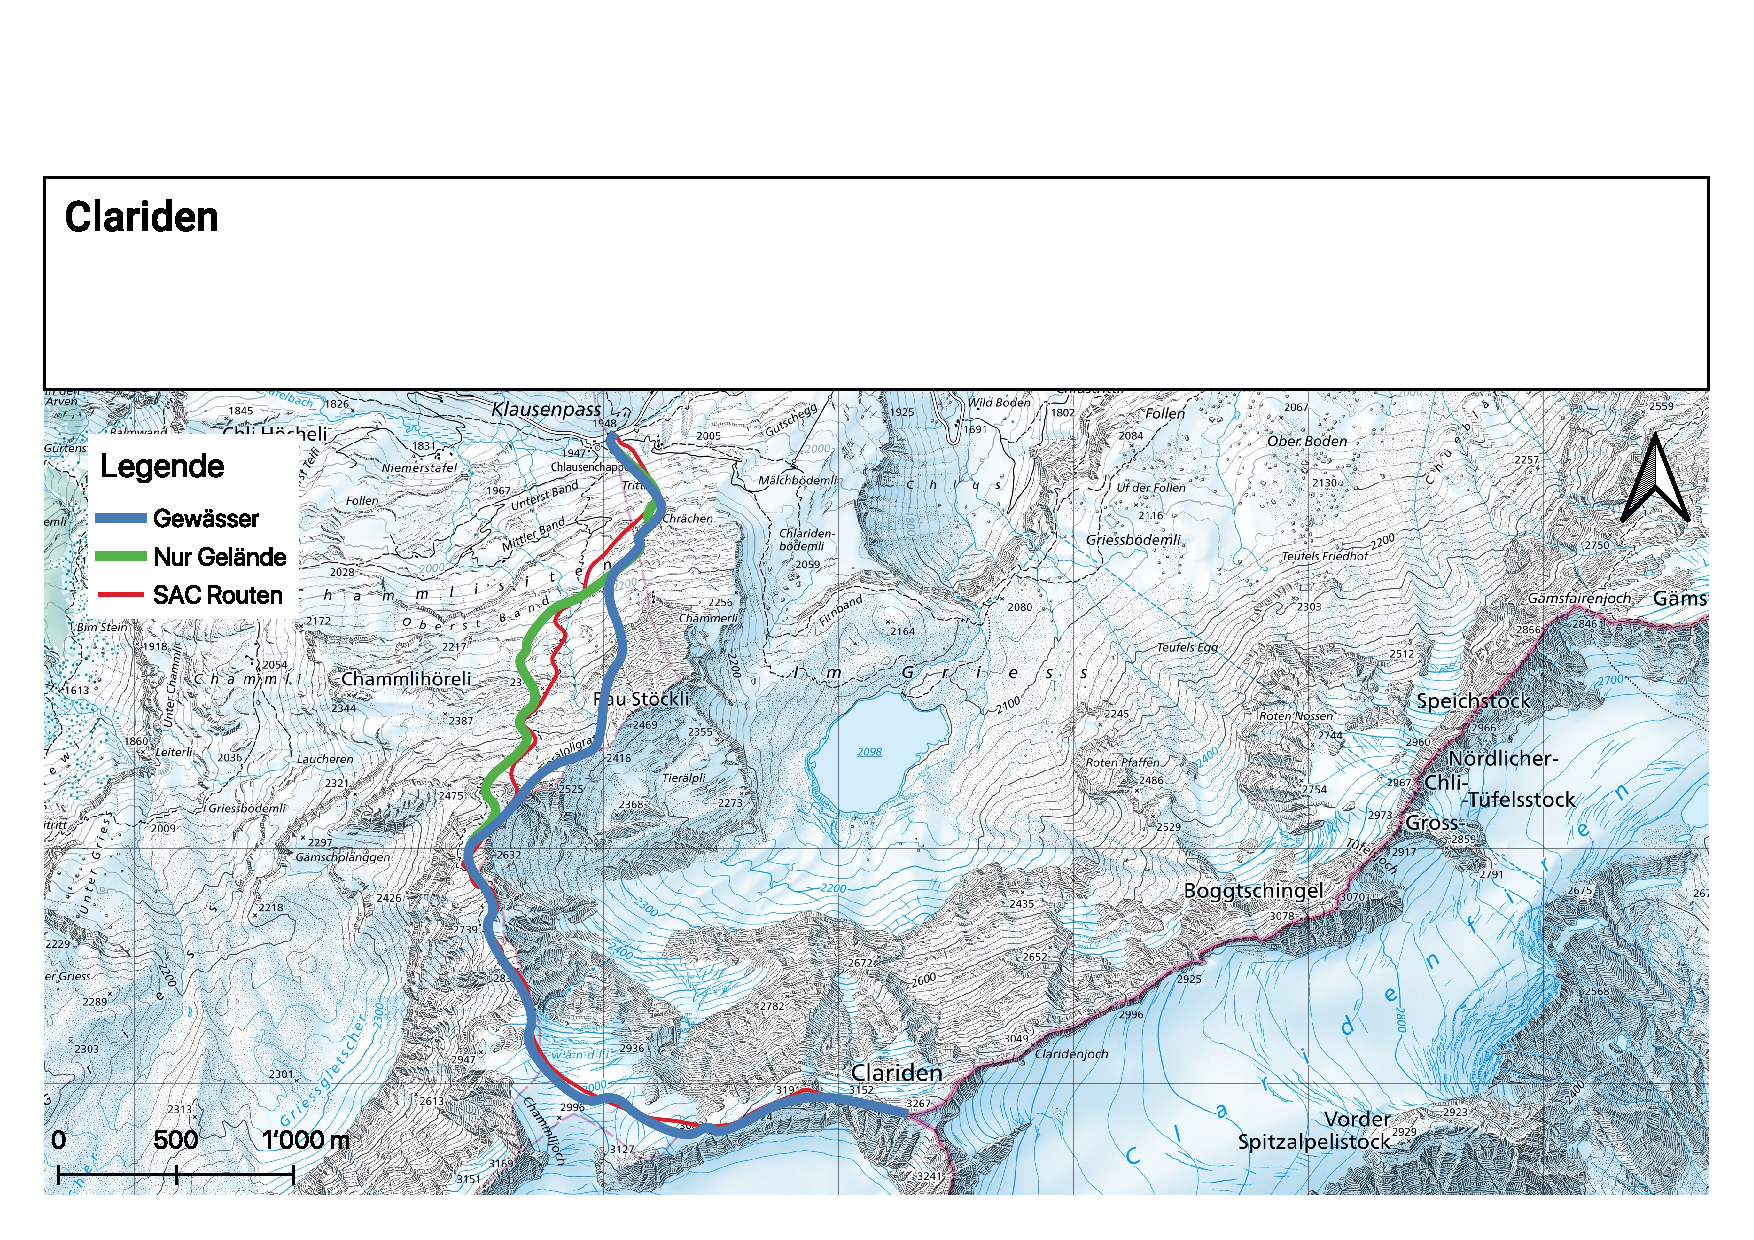
\includegraphics[width=0.8\textwidth, page=1]{PDFs/Clariden.pdf}
\end{center}
% 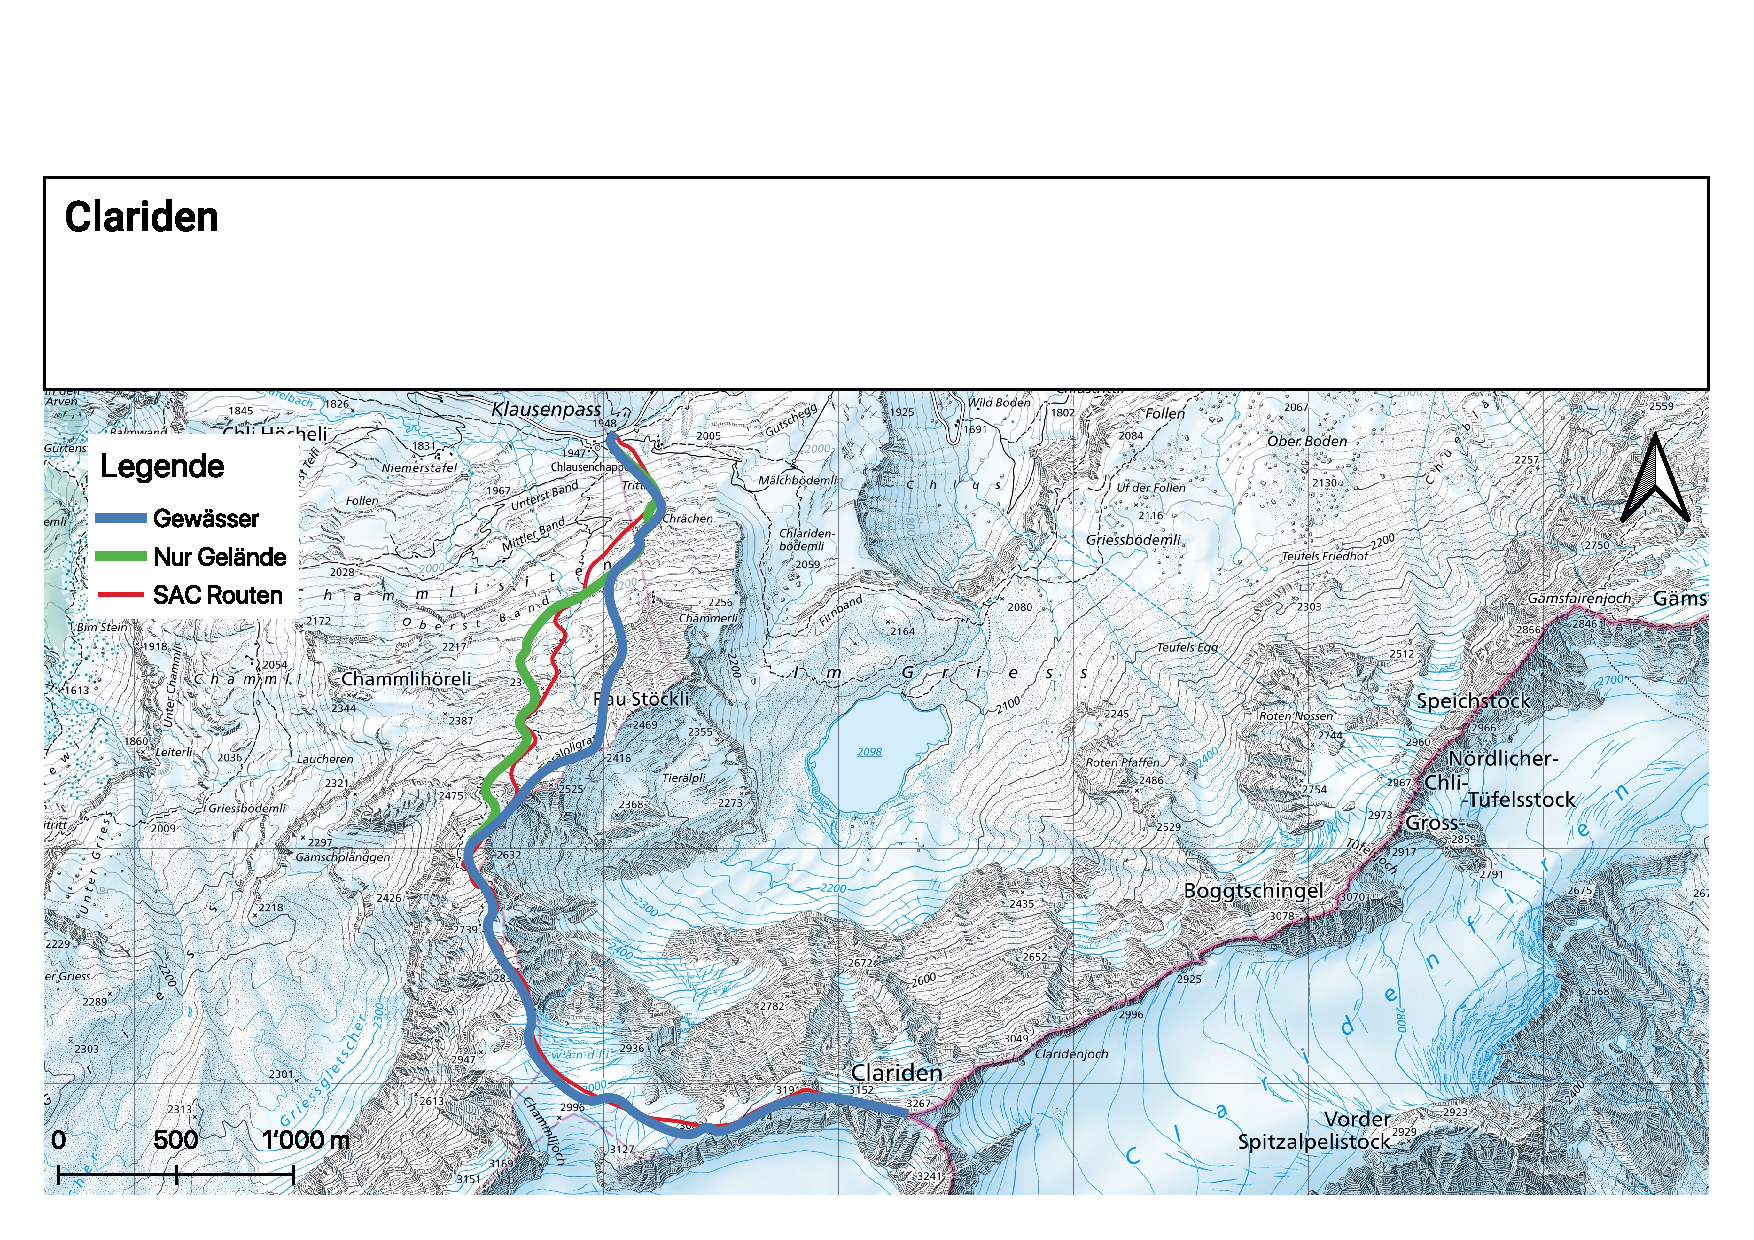
\includepdf[landscape=false, height=7.5cm]{PDFs/Clariden.pdf}

\end{document}